\documentclass[a4paper,UTF8]{article}
%\usepackage{ctex}
\usepackage[margin=1.25in]{geometry}
\usepackage{color} 
\usepackage{graphicx}
\usepackage{amssymb}
\usepackage{amsmath}
\usepackage{amsthm}
\usepackage{enumerate}
\usepackage{bm}
\usepackage{hyperref}
\usepackage{epsfig}
\usepackage{color}
\usepackage{mdframed}
\usepackage{lipsum}
\usepackage{mathtools}
\usepackage{algorithm}
\usepackage{algorithmic}
\usepackage{listings}
\usepackage[usenames,dvipsnames]{xcolor}
\definecolor{mygreen}{rgb}{0,0.6,0}
\definecolor{mygray}{rgb}{0.5,0.5,0.5}
\definecolor{mymauve}{rgb}{0.58,0,0.82}
\lstset{
 basicstyle = \footnotesize,       
 breakatwhitespace = false,        
 breaklines = true,                 
 captionpos = b,                    
 commentstyle = \color{mygreen}\bfseries,
 extendedchars = false,             
 %frame =shadowbox, 
 framerule=0.5pt,
 keepspaces=true,
 keywordstyle=\color{blue}\bfseries, % keyword style
 language = Python,                       % the language of code
 otherkeywords={string}, 
 numbers=left, 
 numbersep=5pt,
 numberstyle=\tiny\color{mygray},
 rulecolor=\color{black},         
 showspaces=false,  
 showstringspaces=false, 
 showtabs=false,    
 stepnumber=1,         
 %stringstyle=\color{mymauve},        % string literal style
 tabsize=2,          
 title=\lstname                      
}
\newmdtheoremenv{thm-box}{myThm}
\newmdtheoremenv{prop-box}{Proposition}
\newmdtheoremenv{def-box}{define}

\setlength{\evensidemargin}{.25in}
\setlength{\textwidth}{6in}
\setlength{\topmargin}{-0.5in}
\setlength{\topmargin}{-0.5in}
% \setlength{\textheight}{9.5in}
%%%%%%%%%%%%%%%%%%set header and footer here%%%%%%%%%%%%%%%%%%
\usepackage{fancyhdr}                                
\usepackage{lastpage}                                           
\usepackage{layout}                                             
\footskip = 10pt 
\pagestyle{fancy}                    
\lhead{2024, Spring}                    
\chead{Computer Vision: Representation and Recognition}
\rhead{Assignment 3}                                                                                               
\cfoot{\thepage}                                                
\renewcommand{\headrulewidth}{1pt}  			%header
\setlength{\skip\footins}{0.5cm}    			
\renewcommand{\footrulewidth}{0pt}  		

\makeatletter 							
\def\headrule{{\if@fancyplain\let\headrulewidth\plainheadrulewidth\fi%
\hrule\@height 1.0pt \@width\headwidth\vskip1pt	
\hrule\@height 0.5pt\@width\headwidth  			
\vskip-2\headrulewidth\vskip-1pt}      			
 \vspace{6mm}}     						
\makeatother  

%%%%%%%%%%%%%%%%%%%%%%%%%%%%%%%%%%%%%%%%%%%%%%
\numberwithin{equation}{section}
\newtheorem{myThm}{myThm}
\newtheorem*{myDef}{Definition}
\newtheorem*{mySol}{Solution}
\newtheorem*{myProof}{Proof}
\newcommand{\indep}{\rotatebox[origin=c]{90}{$\models$}}
\newcommand*\diff{\mathop{}\!\mathrm{d}}

\usepackage{multirow}
\renewcommand\refname{reference}


\begin{document}
\title{Computer Vision: Representation and Recognition\\
	Assignment 3}
\author{211240076, Liu Jiaxin, \href{211240076@smail.nju.edu.cn}{211240076@smail.nju.edu.cn}}
\maketitle

\section{Question 1}

\subsection{question1.1}
\begin{lstlisting}
	def get_correspondences(img1, img2, num_points=4)
\end{lstlisting}
takes the addresses of two images and returns the coordinates of selected points.
plt.ginput is used to get the coordinates of selected points.

\subsection{question1.2}
We assume $\textbf{H}$ is the homography matrix, i.e.
\begin{equation}
	\lambda \textbf{p}=\textbf{H}\textbf{p}'
\end{equation}
\begin{equation}
	\lambda\begin{bmatrix}
		x' \\
		y' \\
		1
	\end{bmatrix}
	=
	\begin{bmatrix}
		h_{11} & h_{12} & h_{13} \\
		h_{21} & h_{22} & h_{23} \\
		h_{31} & h_{32} & h_{33}
	\end{bmatrix}
	\begin{bmatrix}
		x \\
		y \\
		1
	\end{bmatrix}
\end{equation}
Eliminate $\lambda$, set $h_{33}=1$, we have
\begin{equation}
	\begin{bmatrix}
		x & y & 1 & 0 & 0 & 0 & -xx' & -yx' \\
		0 & 0 & 0 & x & y & 1 & -xy' & -yy'
	\end{bmatrix}\begin{bmatrix}
		h_{11} \\
		h_{12} \\
		h_{13} \\
		h_{21} \\
		h_{22} \\
		h_{23} \\
		h_{31} \\
		h_{32}
	\end{bmatrix}=\begin{bmatrix}
		x' \\
		y'
	\end{bmatrix}
\end{equation}
We assume $$\textbf{A}=\begin{bmatrix}
		x & y & 1 & 0 & 0 & 0 & -xx' & -yx' \\
		0 & 0 & 0 & x & y & 1 & -xy' & -yy'
	\end{bmatrix},$$
$$\textbf{x}=\begin{bmatrix}
		h_{11} \\
		h_{12} \\
		h_{13} \\
		h_{21} \\
		h_{22} \\
		h_{23} \\
		h_{31} \\
		h_{32}
	\end{bmatrix},$$
$$\textbf{b}=\begin{bmatrix}
		x' \\
		y'
	\end{bmatrix}$$
The function
\begin{lstlisting}
		def compute_homography_paras(pt1, pt2):
\end{lstlisting}
uses np.linalg.lstsq to solve it and get the homography matrix.
\begin{lstlisting}
	def verify_H(img1, img2, H)
\end{lstlisting}
To verify the homography matrix we compute, we can simply choose point in image1, apply $\textbf{H}$ on it and see if the corresponding point is correct or not.

\subsection{question1.3}
\begin{lstlisting}
	def warp_between_planes(img1_path, H)
\end{lstlisting}
takes the recovered homography matrix and an image, and returns a new image that is the warp of the input image using H we computed before. \\
Here I use np.meshgrid to compute the coordinates for the grid. Then I map the grid using H and get the bounding box of the warped image.
\begin{lstlisting}
	x, y = np.meshgrid(np.arange(w), np.arange(h))
	coords = np.stack([x.flatten(), y.flatten(), np.ones_like(x.flatten())], axis=1)
	# Apply the homography transformation to the grid
    new_coords = (H @ coords.T).T # shape: (.., 3)
\end{lstlisting}
\begin{figure}[H]
	\centering  %centering image
	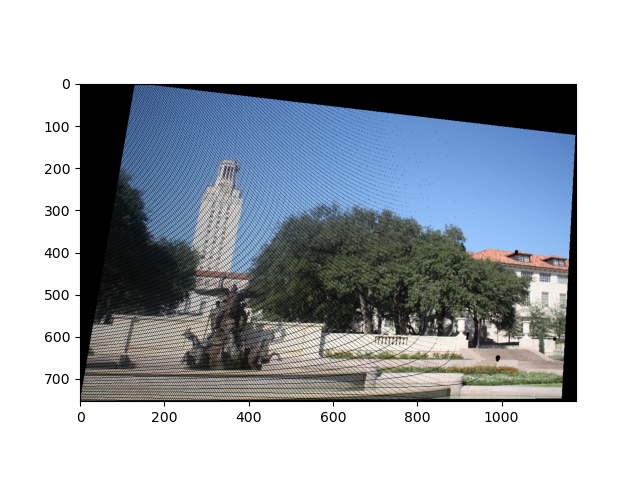
\includegraphics[width=12cm,height=12cm]{warped_img_without_inverse_warp.png}  % load image
	\caption{warped image without inverse warp}  %
\end{figure}
then I interpolate the pixel values in the warped image. \\
In order to avoid holes in the output, an inverse warp is used to fill in the black area. Result is shown as follows:
\begin{figure}[H]
	\centering  %centering image
	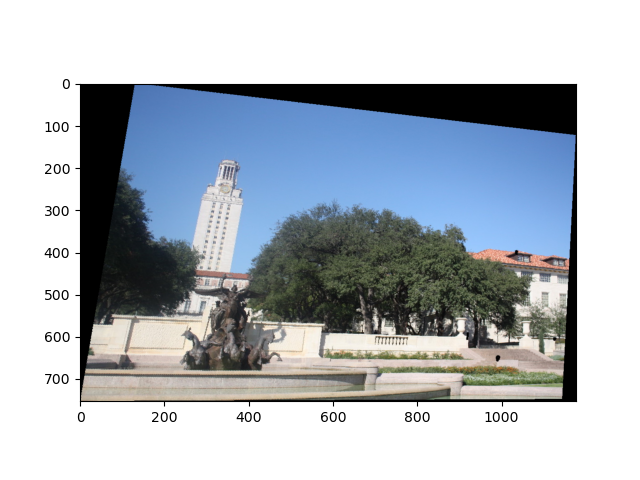
\includegraphics[width=12cm,height=12cm]{warped_img_with_inverse_warp.png}  % load image
	\caption{warped image with inverse warp}  %
\end{figure}

\subsection{question1.4}
The function
\begin{lstlisting}
	def merge_images(warped_image, boundingbox, img2_path)
\end{lstlisting}
creates a merged image showing the mosaic. Specifically, this function combined the warpped image and the original second image

\subsection*{(1) Apply your system to the provided pair of images, and display the output mosaic.}
See "output mosaic1"
\begin{figure}[H]
	\centering  %centering image
	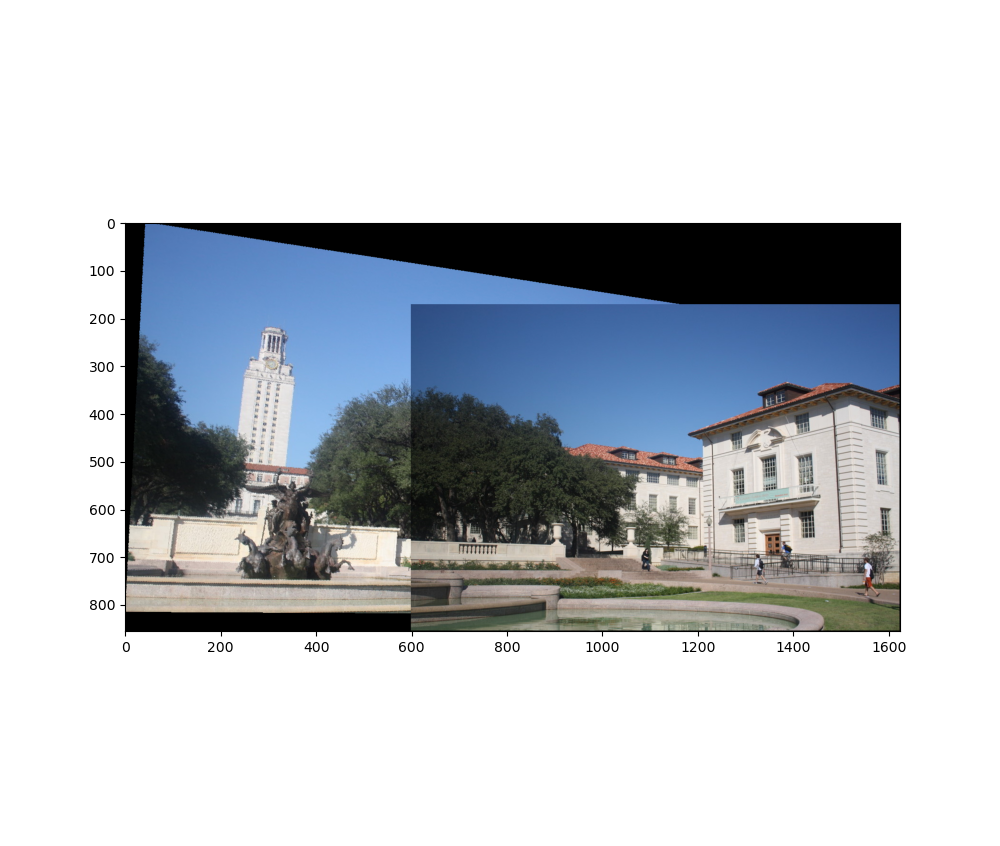
\includegraphics[width=12cm,height=12cm]{result1.png}  % load image
	\caption{output mosaic1}  %
\end{figure}
\subsection*{(2) Show one additional example}
See "output mosaic2"
\begin{figure}[H]
	\centering  %centering image
	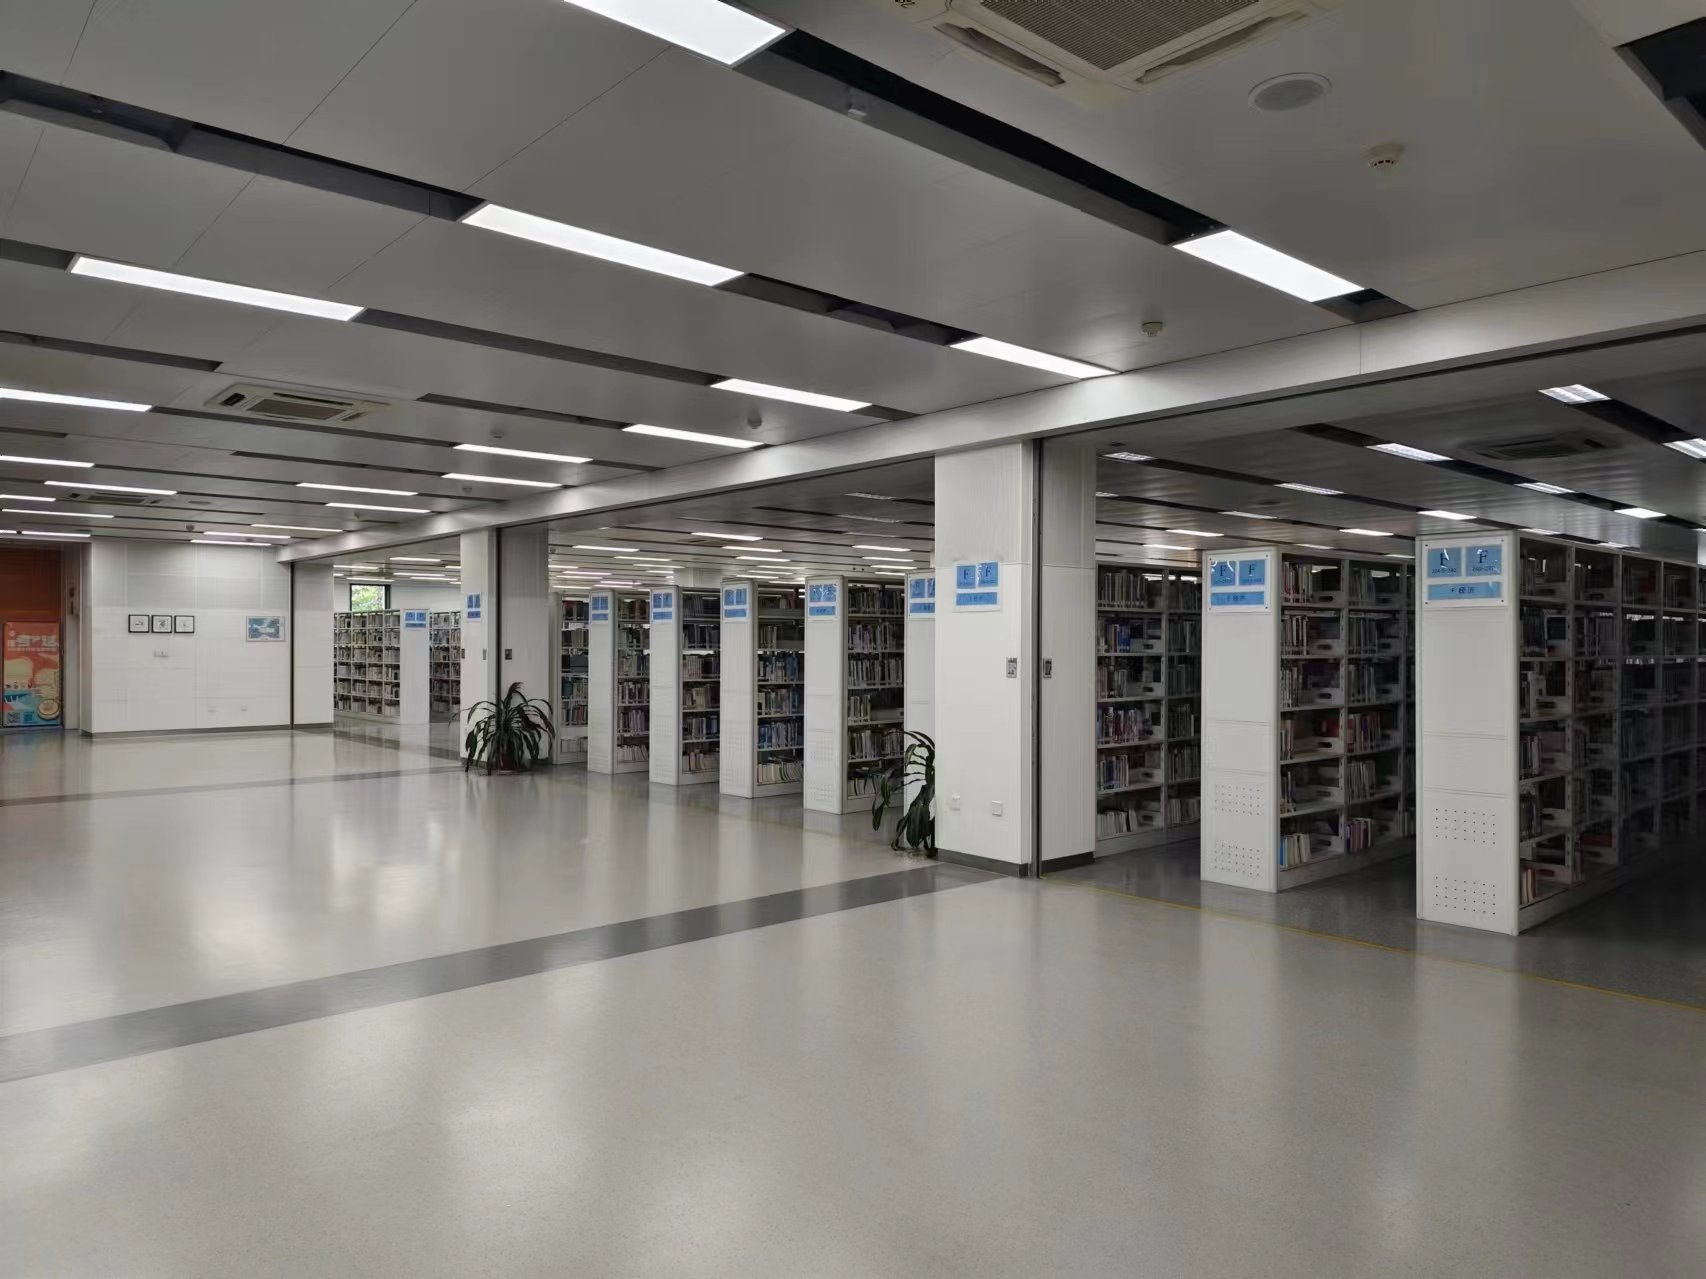
\includegraphics[width=5cm,height=5cm]{img1.jpg}  % load image
	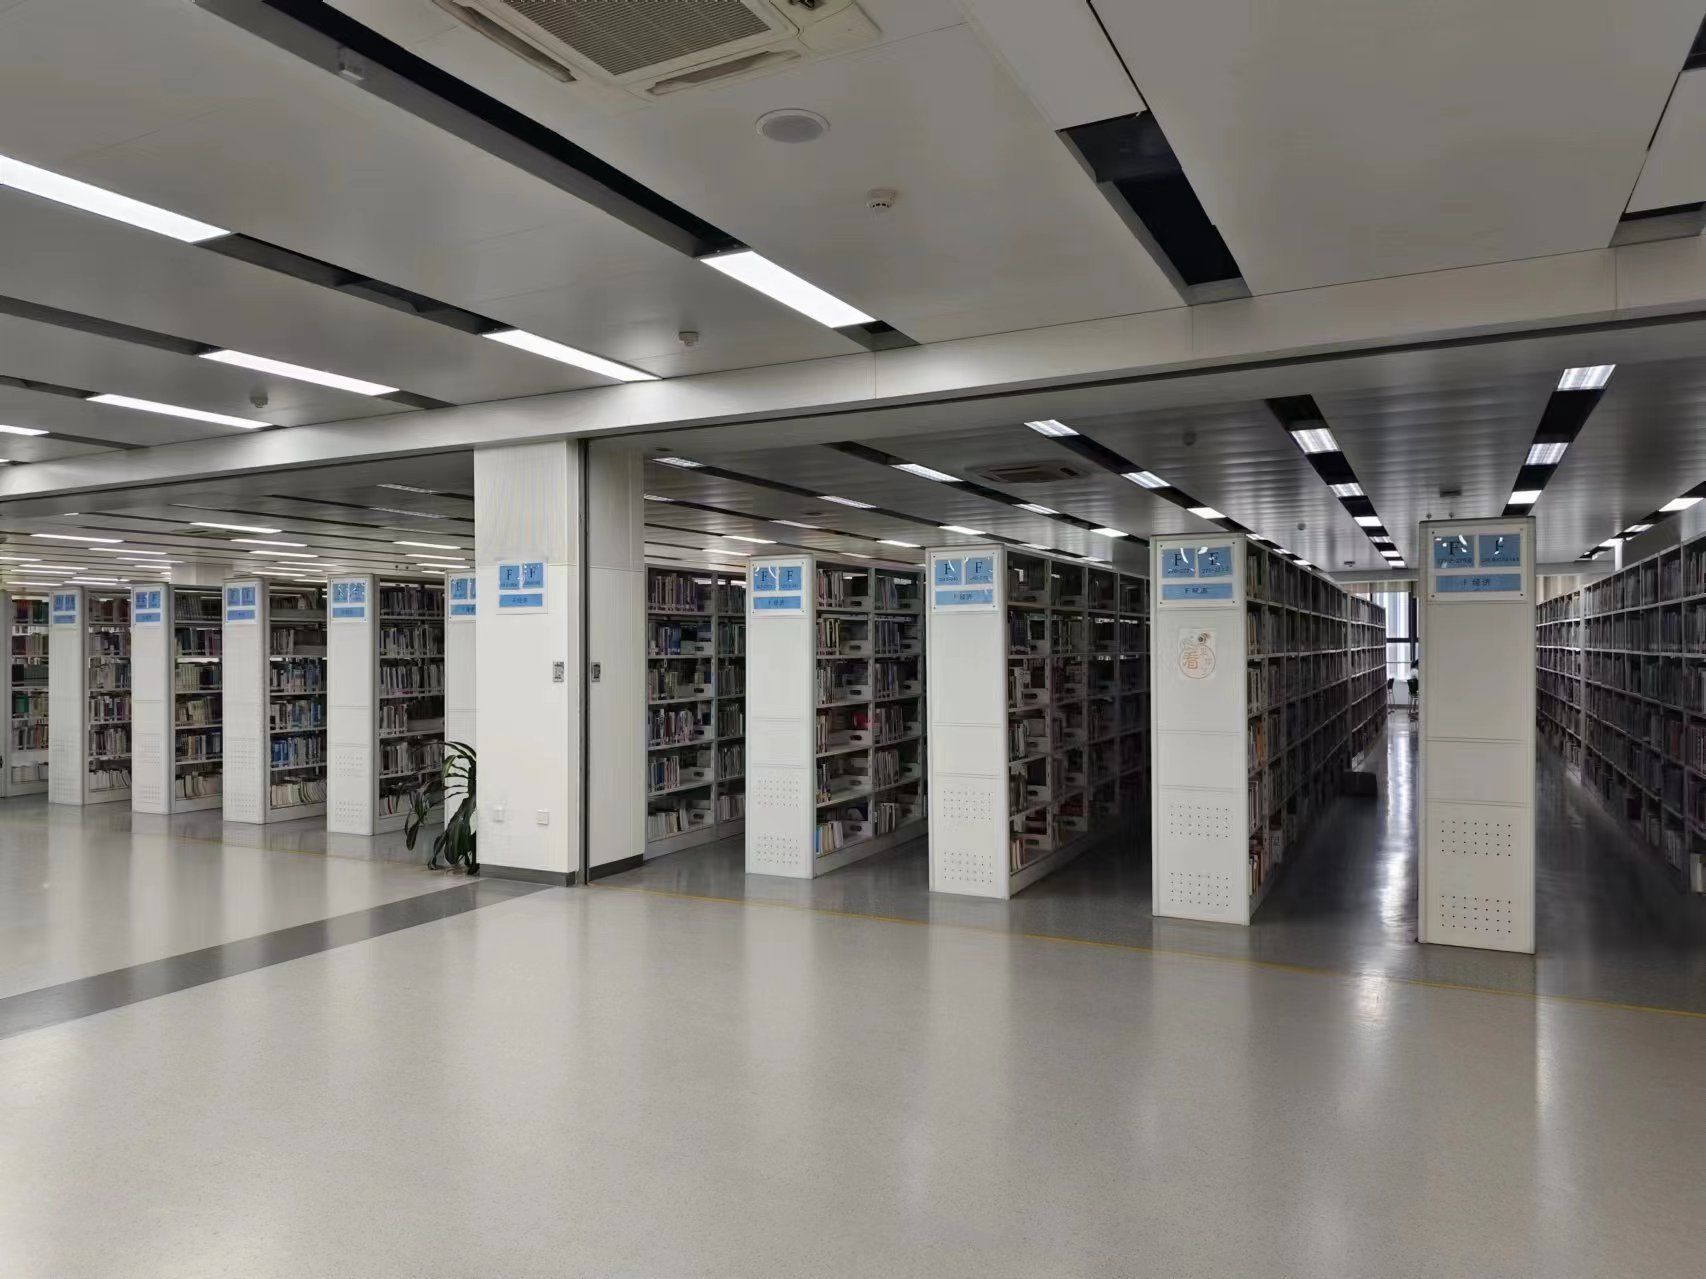
\includegraphics[width=5cm,height=5cm]{img2.jpg}  % load image
	\caption{images used}  %
\end{figure}
\begin{figure}[H]
	\centering  %centering image
	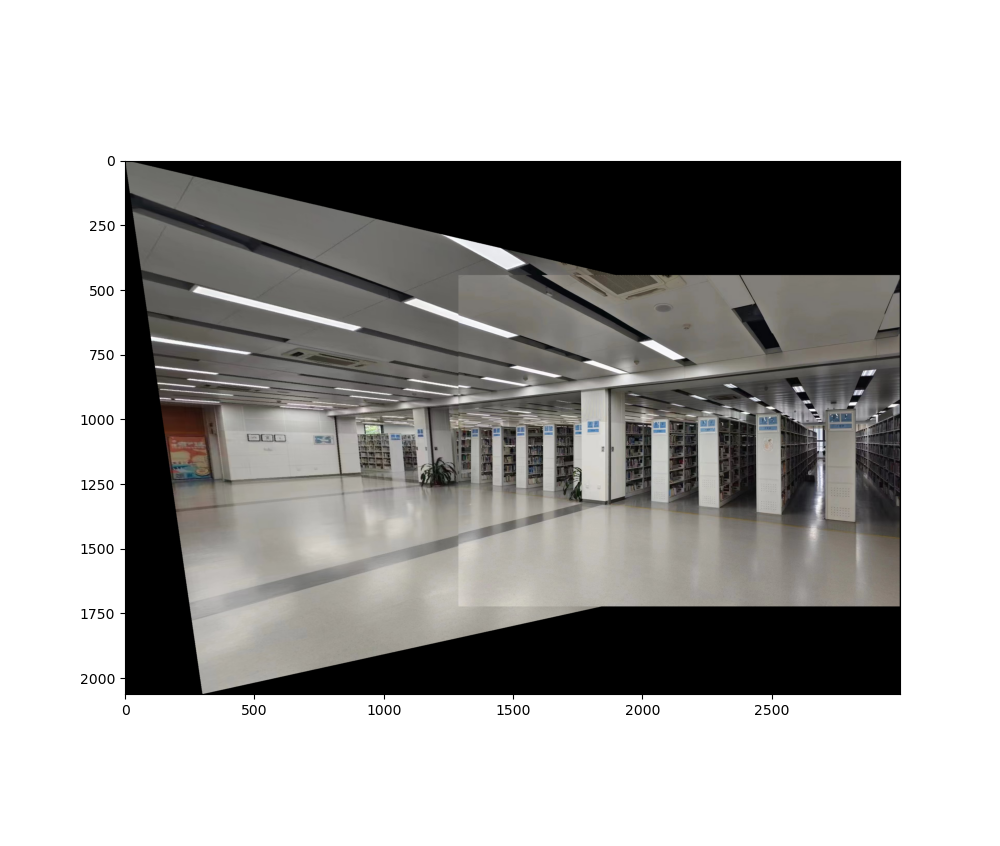
\includegraphics[width=12cm,height=12cm]{result2.png}  % load image
	\caption{output mosaic2}  %
\end{figure}
\subsection*{(3) Warp one image into a "frame" region}
We can warp the image to the frame by clicking the points of the frame and the four corners of the desired image. \\
Notice we should overwrite the frame image. So we need to switch the order in the function merge\_images
\begin{lstlisting}
    for j in range(img2.shape[0]):
        for i in range(img2.shape[1]):
            merged_image[j-y_zero][i-x_zero] = img2[j][i]
	for j in range(warped_image.shape[0]):
		for i in range(warped_image.shape[1]):
			if np.any(warped_image[j][i]): ## don't write black pixel
				merged_image[j+min_y-y_zero][i+min_x-x_zero] = warped_image[j][i]
\end{lstlisting}
\begin{figure}[H]
	\centering  %centering image
	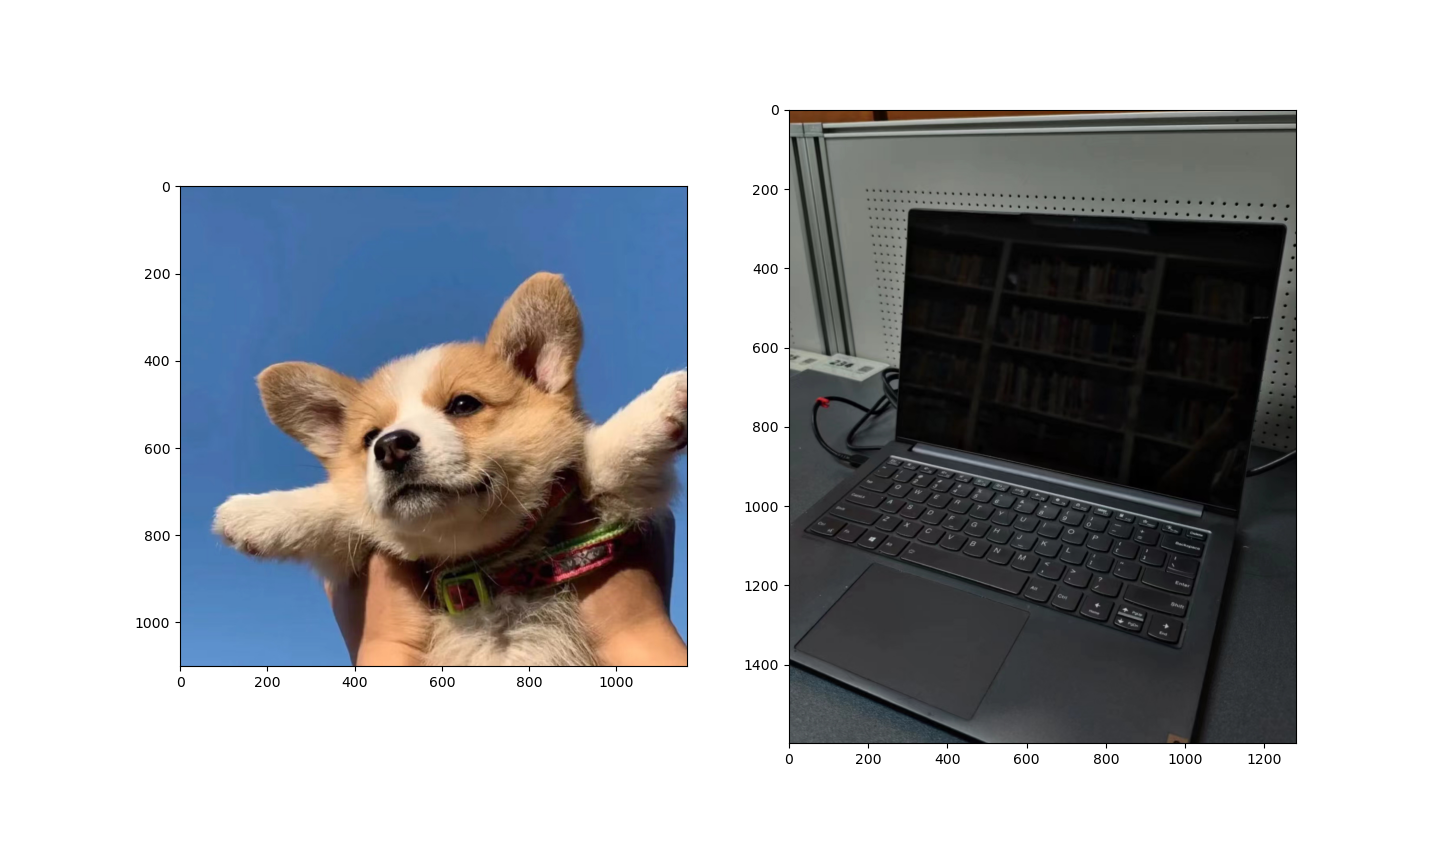
\includegraphics[width=1\textwidth]{frame_plot.png}  % load image
	\caption{frame and image}  %
\end{figure}
\begin{figure}[H]
	\centering  %centering image
	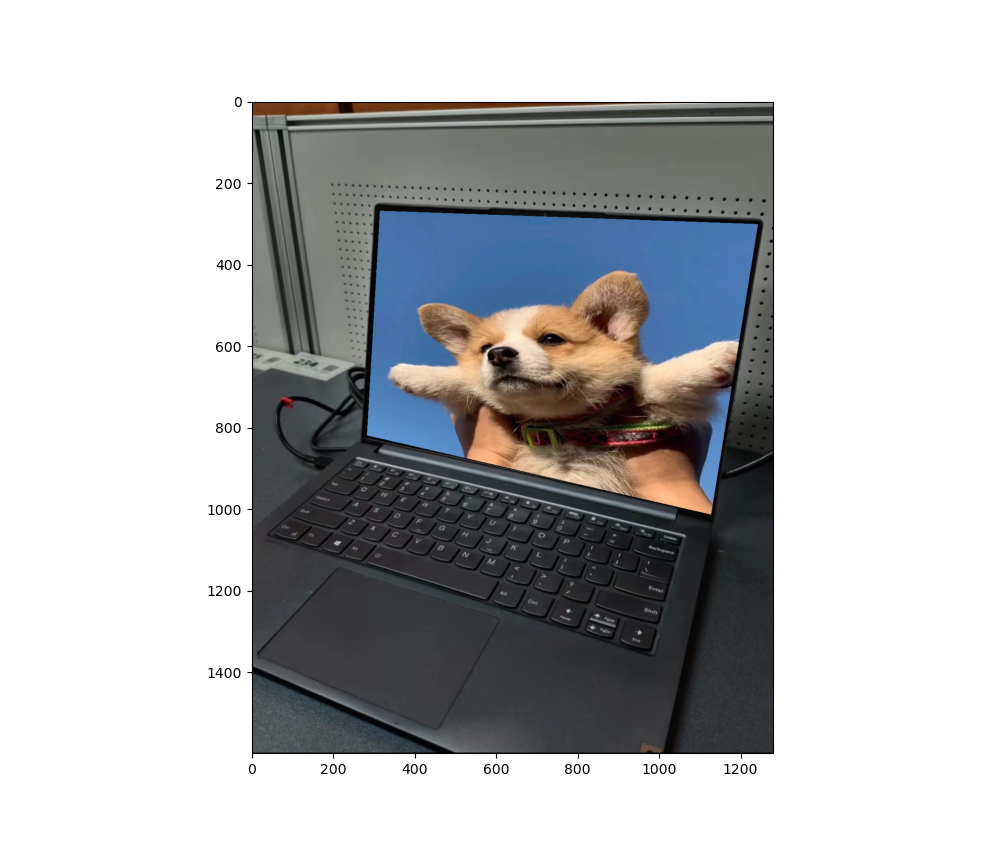
\includegraphics[width=11cm,height=11cm]{frame_merged.png}  % load image
	\caption{Output image}  %
\end{figure}

\section{Question 2}

\subsection{question2.1}
The function
\begin{lstlisting}
	def get_correspondences_sift(image1, image2)
\end{lstlisting}
uses sift to automatically identify matching descriptors in the two input images. \\
Specifically, it first converts two images into grayscale and compute SIFT keypoints and descriptors for both images. Then it finds matching descriptors using brute-force matching.
After that, ratio test is applied to filter good matches. SO we can get the desired correspondences.
\begin{figure}[H]
	\centering  %centering image
	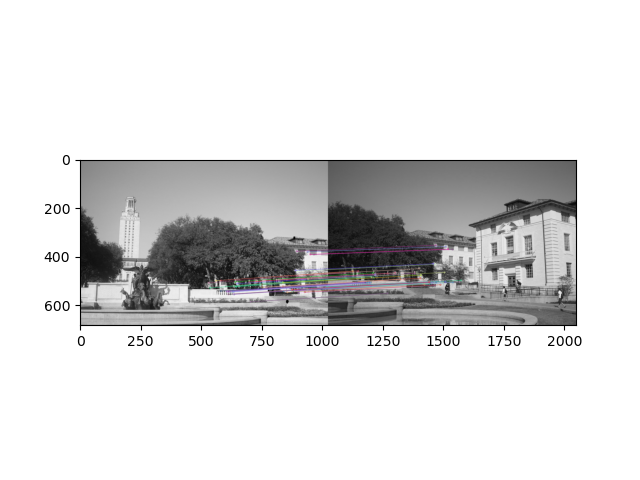
\includegraphics[width=1\textwidth]{sift.png}  % load image
	\caption{automatically obtain interest points and descriptors with SIFT}  %
\end{figure}
Reusing the codes (still use compute\_homography\_paras(pt1, pt2) to compute homography matrix H), we can get the results:
\begin{figure}[H]
	\centering  %centering image
	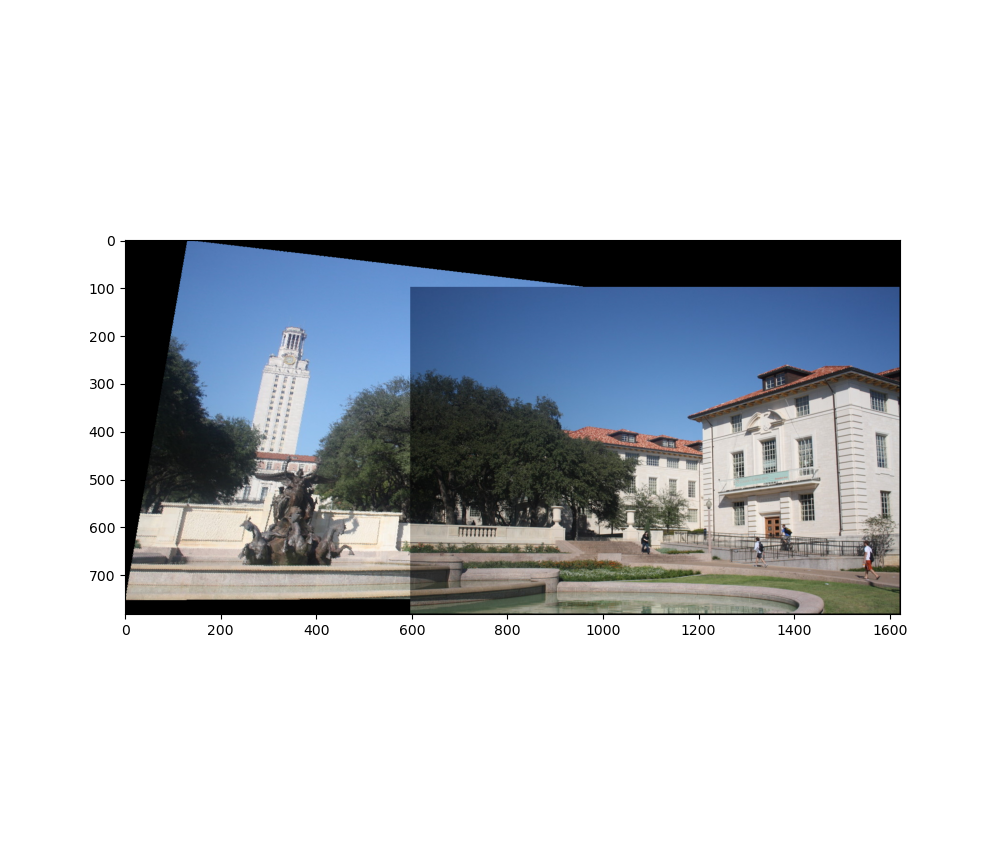
\includegraphics[width=12cm,height=12cm]{result_auto1.png}  % load image
	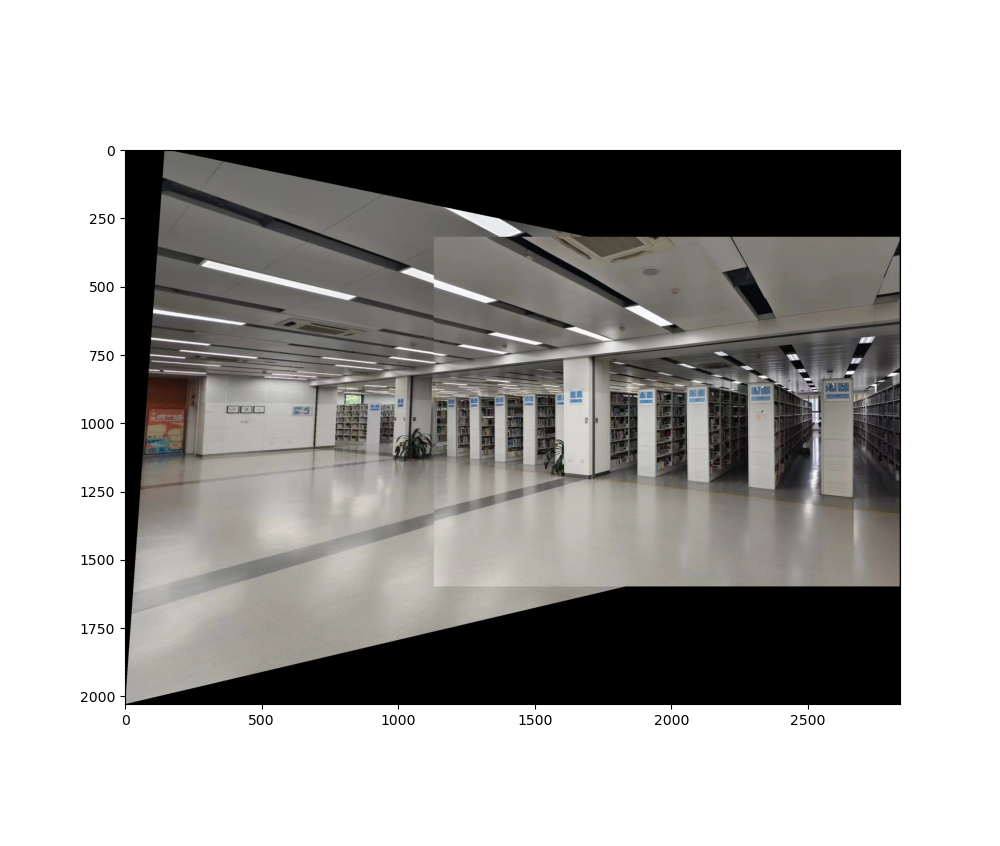
\includegraphics[width=12cm,height=12cm]{result_auto2.png}  % load image
	\caption{results using SIFT}  %
\end{figure}
\subsection{question2.2}
\begin{lstlisting}  
	# ordinary method RANSAC (4th parameters should be in [1, 10])
    H, mask = cv2.findHomography(np.asarray(pt1), np.asarray(pt2), 0, 5.0)
    # RANSAC
    H, mask = cv2.findHomography(np.asarray(pt1), np.asarray(pt2), cv2.RANSAC, 5.0)
\end{lstlisting}
Below figures shows the difference between whether or not using RANSAC.
\begin{figure}[H]
	\centering  %centering image
	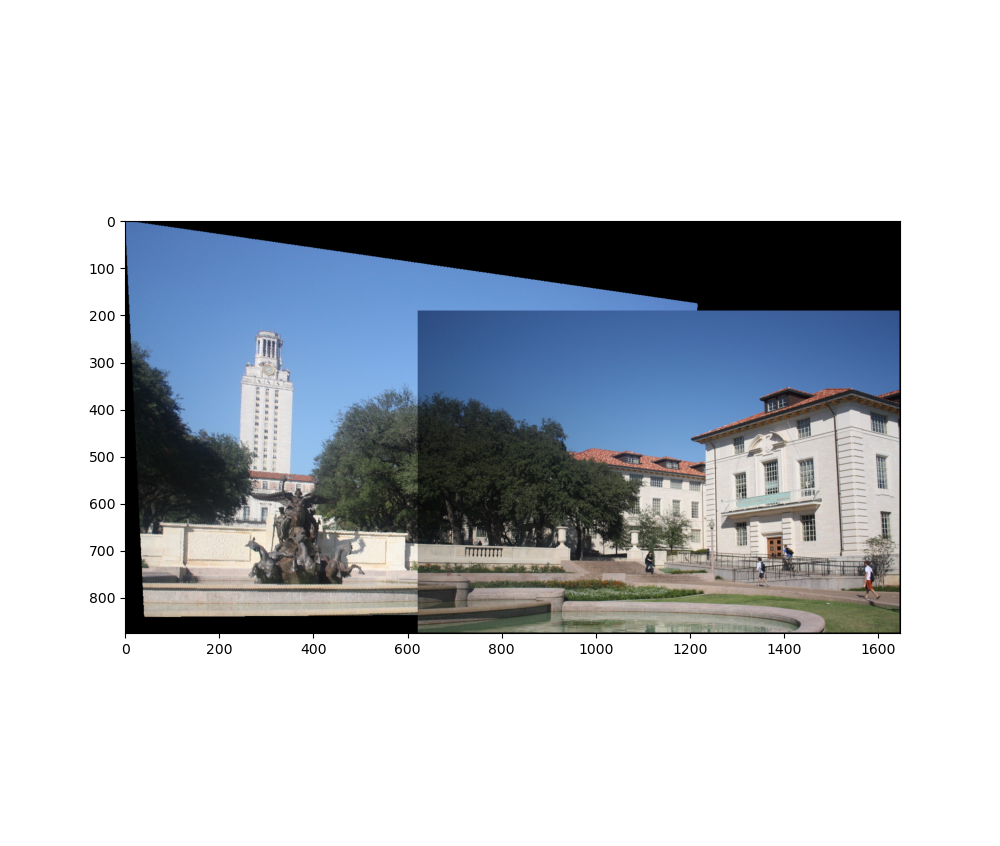
\includegraphics[width=8cm,height=8cm]{wo_RANSAC.png}  % load image
	\caption{results without using RANSAC}  %
\end{figure}
\begin{figure}[H]
	\centering  %centering image
	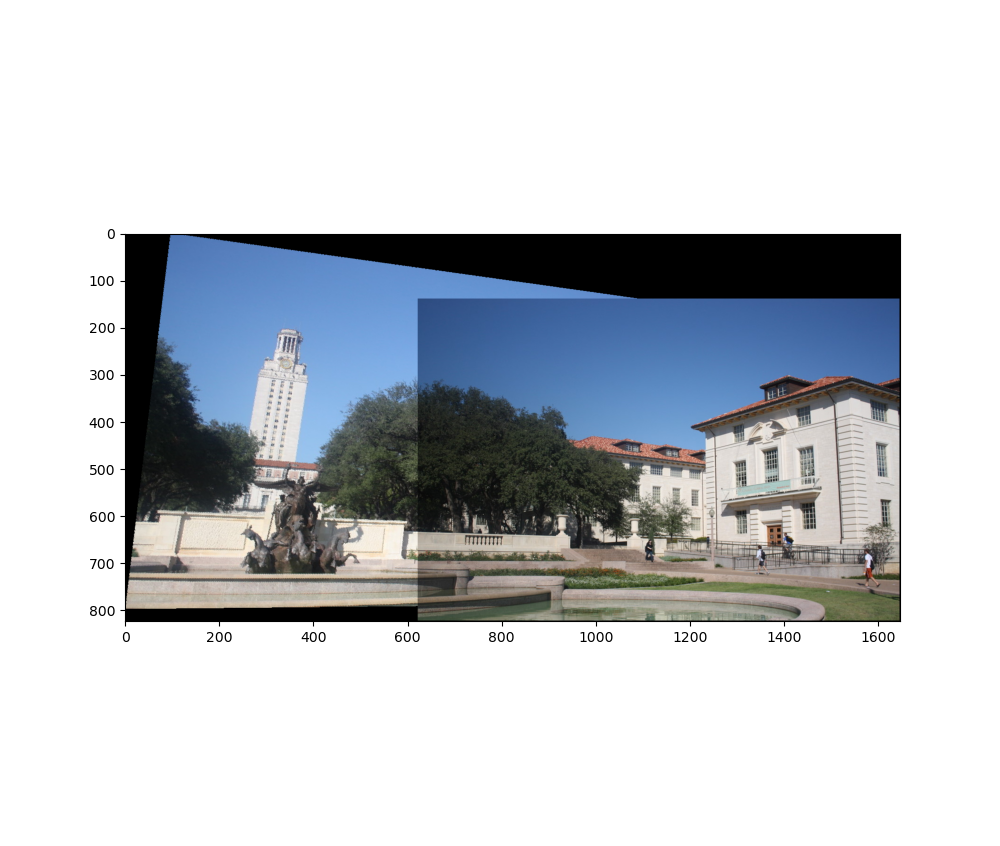
\includegraphics[width=8cm,height=8cm]{with_RANSAC.png}  % load image
	\caption{results using RANSAC}  %
\end{figure}
We can see in this case RANSAC slightly improves the alignment, since RANSAC removes some outliers.
Here are more obvious results showing the advantages of RANSAC:
\begin{figure}[H]
	\centering  %centering image
	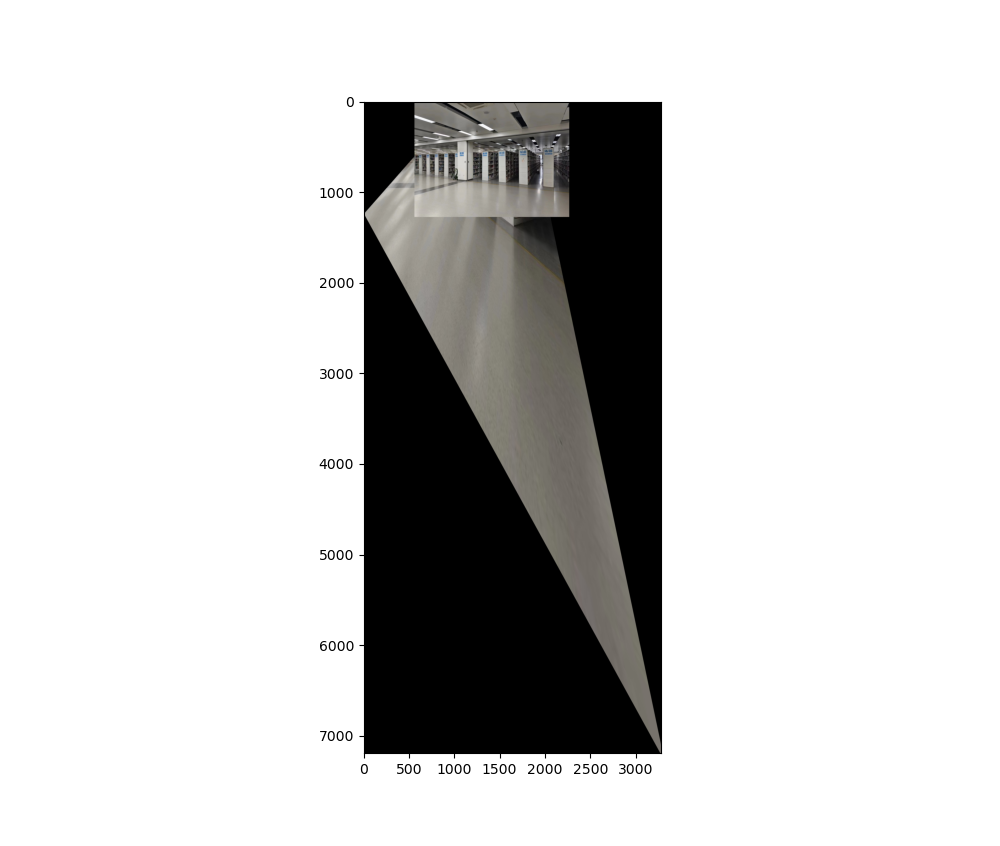
\includegraphics[width=12cm,height=12cm]{wo_RANSAC2.png}  % load image
	\caption{another result without using RANSAC}  %
\end{figure}
We see that the mosaic image is pretty worse. That is because some outliers make bad influence on the output.
\begin{figure}[H]
	\centering  %centering image
	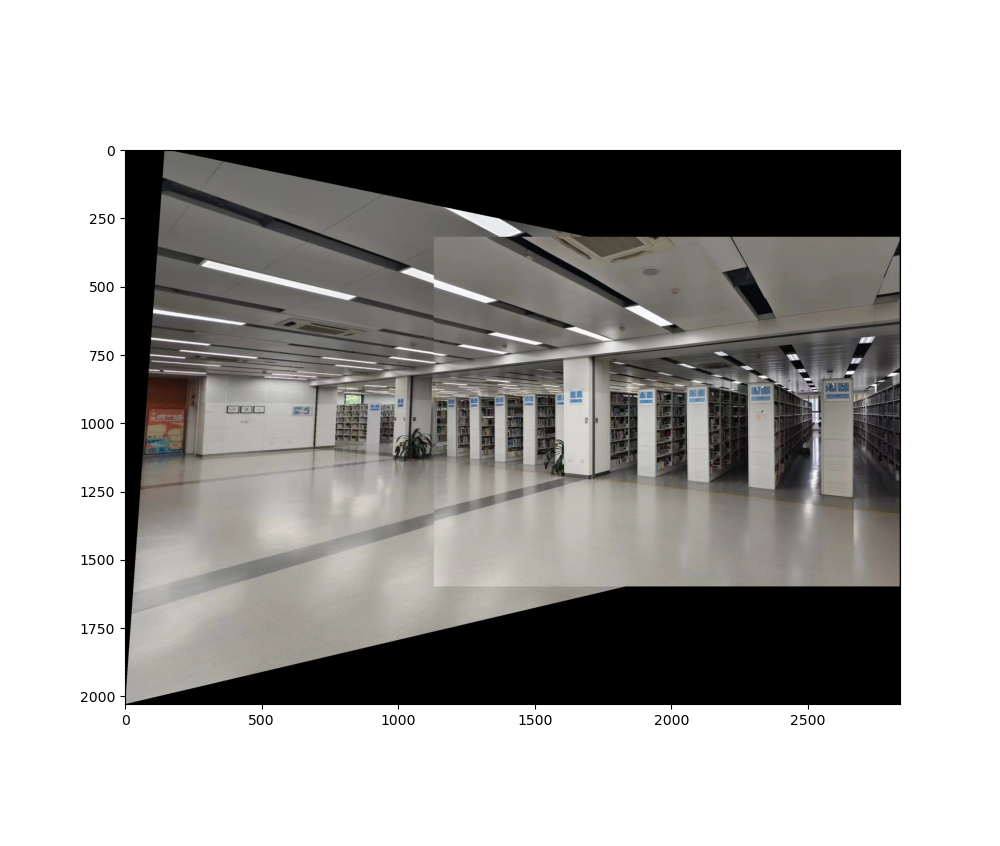
\includegraphics[width=8cm,height=8cm]{with_RANSAC2.png}  % load image
	\caption{another result using RANSAC}  %
\end{figure}
\bibliographystyle{plain}
\bibliography{ref}
\end{document}